\documentclass[border=4pt]{standalone}
\usepackage{tikz}
\usetikzlibrary{shapes.symbols,positioning,arrows.meta}

\begin{document}
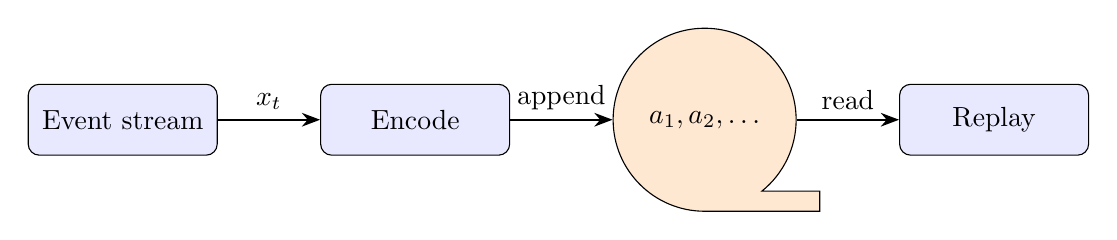
\begin{tikzpicture}[
  >=Stealth,
  node distance=13mm,
  stage/.style={draw,rounded corners,minimum width=24mm,minimum height=9mm,fill=blue!9},
  store/.style={magnetic tape,draw,minimum size=17mm,magnetic tape tail=.22,
    magnetic tape tail extend=3mm,fill=orange!18},
  flow/.style={->,thick}
]
  \node[stage] (events) {Event stream};
  \node[stage,right=of events] (encode) {Encode};
  \node[store,right=of encode] (archive) {$a_1,a_2,\ldots$};
  \node[stage,right=of archive] (query) {Replay};

  \draw[flow] (events) -- node[above]{$x_t$} (encode);
  \draw[flow] (encode) -- node[above]{append} (archive);
  \draw[flow] (archive) -- node[above]{read} (query);
\end{tikzpicture}
\end{document}
